\documentclass[conference,harvard,brazil,english]{sbatex}
\usepackage[utf8]{inputenc}
\usepackage{float}
\usepackage{ae}
\usepackage{amsfonts, amssymb}
\usepackage{amsmath}
\usepackage{graphicx}
\usepackage{indentfirst}
\usepackage{ae}
\usepackage{gensymb}
\usepackage{caption} 
\usepackage{epstopdf}
\usepackage{leading}
\usepackage[table,xcdraw]{xcolor}
\usepackage{tablefootnote}

\usepackage{natbib}
\bibliographystyle{dinat}

\makeatletter
\def\verbatim@font{\normalfont\ttfamily\footnotesize}
\makeatother
\usepackage{amsmath}
% --------------------------------------------------
\begin{document}
    \title{Síntese de Controladores Digitais para um Sistema de Controle de Posição de um Motor}
    \author{Marcus Vinícius de Oliveira Gama}{marcusgamacefet@gmail.com}
    \author{ Thalles Oliveira Campagnani}{thallescampagnani@gmail.com}
    %--------------------------------
    \twocolumn[
        \maketitle
        \selectlanguage{brazil}
        \nocite{nise}
        \nocite{DB95}
        \begin{abstract}
            O presente trabalho apresenta a identificação do modelo do processo relacionado a posição angular do motor, sintetiza dois controladores diferentes por meio de técnicas do controle clássico (PID) e do controle moderno (Espaço de Estados Estimados), realiza a analise dos sistemas em malha fechada, e compara os resultados.
        \end{abstract}
        \keywords{Controle de Posição de um Motor, Controlador PID, Controlador no Espaço de Estados.}
        \selectlanguage{english}
        \begin{abstract}
            The present work presents the identification of the process model related to the angular position of the motor, synthesizes two different controllers using classical control (PID) and modern control (State Space) techniques, and compare the results.
        \end{abstract}
        \keywords{Motor Position Control, PID Controller, State Space Controller.}
    ]
    \selectlanguage{brazil}
    %--------------------------------
    
    \section{Introdução}
        
        O motor de corrente continua é um integrador natural, tornando impossível ser controlada sua posição em malha aberta. Para realizar o controle de posição é necessário sensoreá-la e fechar a malha de controle com um controlador projetado para atingir determinado desempenho.
        
        %Os controladores podem ser implementados em microcontroladores, neste caso faz-se necessário analisar o efeito da discretização do sinal no  sistema.
        
        As abordagens escolhidas no projeto dos controladores foram a Realimentação de Estados Estimados, REE, e o controlador Proporcional Integrativo e Derivativo, PID, a fim de comparar uma técnica de controle clássico com uma técnica de controle moderno.
        
        A metodologia de projeto consiste em, nesta ordem: se definir critérios de desempenho desejados para o sistema de malha fechada, os polos de dinâmica dominante, a taxa de amostragem que atenda esses critérios de desempenho, a transformação do plano \textit{s} para o plano \textit{z}, e por fim fazer uso das técnicas de síntese de controladores.
        
    \section{Objetivos}
        
        \subsection{Objetivos Gerais}
            
            O presente trabalho tem o objetivo de implementar controladores ensinados na disciplina de Controle Digital em uma planta física, a fim de demonstrar a compreensão dos métodos e a eficácia dos mesmos aplicados dentro de um sistema real.
        
        \subsection{Objetivos Específicos}
            
            Os controladores devem ser sintetizados de forma, que em sua análise de desempenho em malha fechada, se utilize o sinal de controle disponível em toda sua extensão para uma variação de $\pm35\degree$.
    
    \section{Fundamentação Teórica}
        
        \subsection{Controlador PID}
        
            O PID é um dos algorítimos de controlador mais usados na indústria. Ele é popular devido a sua ampla gama de utilização, facilidade de implementação, e manutenibilidade.
            
            A componente proporcional atua mediante o erro do sistema. Ela determina a taxa de resposta de saída para o sinal de erro. Em geral, aumentar o ganho proporcional irá aumentar a velocidade de resposta do sistema de controle. No entanto, se for muito grande, o sistema poderá ficar instável.
            
            A componente integral é responsável por ajustar a resposta temporal em regime permanente. Ela faz com que o sinal de controle aumente com o tempo se o erro for maior que zero, o que fará com que o erro de estado estacionário seja nulo além de rejeitar pertubações do tipo degrau.
            
            A componente derivativa é responsável por atuar no regime transiente. Ela faz com que o sinal de controle diminua o erro apresentar uma amplitude de variação grande.
            
            \begin{figure}[!htb] 
            \centering \includegraphics[width=0.5\columnwidth]{imagens/esquemaPID.png}{
                \small
                \centering
                \caption{Esquemático do controlador PID}
                \label{PID_corte}}
            \end{figure}
            
            \subsubsection{Metodologia de Projeto - PID}
            
                Um controlador PID discreto com filtro é descrito pela seguinte equação:
                
                \begin{equation}
                    C(z) = K_p + K_d\frac{z-1}{z+F} + K_i\frac{z}{z-1}
                \end{equation}
                No qual $F$ é a posição do polo referente ao filtro, $K_p$ é o ganho proporcional, $K_d$ é o ganho derivativo, $K_i$ é o ganho integrativo.
                Para $F=0$, ou seja, o PID sem filtro, a equação pode ser desenvolvida como abaixo:
                
                \begin{equation}
                    C(z) = \frac{(K_p + K_d + K_i)z^2 - (K_p + 2K_d)z + Kd} {z(z-1)}
                \end{equation}
                
                Como não existe variáveis no denominador da função, só é possível variar os zeros nesta abordagem, o que simplifica metodologia de projeto.
                
                Um dos zeros é projetado como um compensador em avanço de fase, utilizando o critério de ângulo.
                
                O outro dos zeros é projetado como um compensador em atraso de fase, colocando o zero perto o suficiente para não influenciar no lugar geométrico das raízes.
        
        \subsection{Controlador REE por alocação de Polos}
        
            O controle de sistemas dinâmicos no espaço de estados é realizado por meio da realimentação dos estados do sistema sendo muito mais eficiente e mais potente do que o controle por realimentação das saídas. O grande problema do controle por realimentação dos estados é exigir que os estados do sistema estejam disponíveis para serem realimentados, ou seja, é necessário medir todos os estados do sistema ou pelo menos estimá-los (observador de estados). 
            
            \subsubsection{Metodologia de Projeto - REE}            
            Um sistema regulador de estados consiste em uma malha fechada na qual as referências para as saídas são todas iguais a zero, em sua representação discreta é dada por:
            
            \begin{equation}
                r[k]-y[k]=0
            \end{equation}
           
           Dessa maneira para um sistema representado em espaço de estados por:
           
           \begin{equation}
               \left\{\begin{matrix}
                    \vec{x}[k+1]=A\vec{x}[k]=Bu[k] \\
                    y[k]=C\vec{x}[k]+Du[k]
                \end{matrix}\right.
           \end{equation}
            No qual $x\in \mathbb{R}^{nx1}, u\in\mathbb{R}^{p}$ e $y\in \mathbb{R}^{m}$. Assumindo que este sistema composto por (A, B) seja controlável e composto por (A, C) seja observável o controle por realimentação dos estados é definido por:
           
           \begin{equation}
               u[k]=-K\vec{x}[k]
           \end{equation}
           
           Pode-se determinar a matriz de ganho $K$ de realimentação de estados através da fórmula de Ackermann definida por:
           
           \begin{equation}
                K= \begin{bmatrix}
                    0 & 0 & \cdots & 1
                \end{bmatrix}
                \textbf{C}^{-1}\Delta_d(A)
                \label{ackermann_controla}
           \end{equation}
           
           sendo
           
           \begin{equation}
               \textbf{C}= \begin{bmatrix}
                    B & AB & A^2B & \cdots & A^{n-1}B
               \end{bmatrix}
               \label{controlabilidade}
           \end{equation}
           
           \begin{equation}
               \Delta_d(A)= A^n+\alpha_1A^{n-1}+\cdots+\alpha_{n-1}A+\alpha_nI
           \end{equation}
           com os $\alpha$'s definidos, segundo o Teorema de Cayley-Hamilton, pelo polinômio característico desejado para o sistema de matriz de estados $A$. Da mesma maneira se define a fórmula de Ackermann para o observador:
            
            \begin{equation}
                L=\Delta_d(A)\textbf{O}^{-1}
                \begin{bmatrix}
                    0\\ 
                    0\\ 
                    \vdots\\ 
                    1
                \end{bmatrix}
            \end{equation}
            
            Onde
            
            \begin{equation}
                \textbf{O}=\begin{bmatrix}
                C\\
                CA\\
                CA^2\\
                \vdots\\
                CA^{n-1}
                \end{bmatrix}
            \end{equation}
            
            Na Figura \ref{ss_corte} pode-se observar um esquemático de como é a representação do controlador e observador por REE.
            
            \begin{figure}[!htb] 
            \centering
                \includegraphics[width=0.5\columnwidth]{imagens/esquemaREE.png}{
                \small
                \centering
                \caption{Esquemático do controlador e observador por REE}
                \label{ss_corte}}
            \end{figure}
            
        
    \section{Desenvolvimento}
    
        \subsection{Descrição da Planta}
        
            A planta consiste basicamente em um veículo de duas rodas com um atuador em cada. A primeira delas, atua na velocidade da roda traseira, enquanto o outro controla ângulo de inclinação da roda dianteira, que este ultimo é o processo a ser controlado no escopo deste trabalho, com o objetivo de permitir futuramente que estes dois atuadores juntos controlem também a posição angular da planta em relação a gravidade.
            
            O processo em questão é constituído por um motor com redução, um potenciômetro, uma ponte-H com chip \textit{LN-298}, um microcontrolador \textit{Arduino NANO}, e acoplado o eixo do motor um garfo de roda preso a roda dianteira. O potenciômetro mede a saída do processo, ele atua como divisor de tensão e é conectado ao DAC, conversor analógico para digital, do microcontrolador. Já o motor é a entrada do processo, ele é conectado a ponte H que a mesma é conectada a alimentação e ao microcontrolador.
            
            É sabido que o motor é um integrador natural, partindo da premissa que a dinâmica da planta não é função da saída, qualquer ângulo pode ser ponto de operação. Será escolhido o angulo de 90\degree já que o mesmo será usado futuramente como ponto de operação de outro processo. Partindo da mesma premissa, é possível concluir que a entrada deve ser nula quando a saída esta estacionada na referencia. Logo o ponto de operação é (tensão,ângulo) = (0,0).
            
            \subsubsection{Faixa de valores de entrada}
                
                A entrada do processo de controle de posição angular é a tensão encima do motor de corrente continua, possui engrenagens de redução e rolamentos, resultando em não linearidades no atuador.
                
                A zona morta precisa ser tratada antes de realizar a identificação do atuador, a fim de reduzir as não linearidades. Identificou-se experimentalmente uma zona morta (incluindo o atrito estático) de aproximadamente $\pm 1.236V$. Este valor é somado em modulo ao sinal de controle (via código) quando é diferente de 0, logo a saturação do sinal de controle em bits é reduzida, enquanto a tensão real é mantida. Apesar do tratamento, o ponto de operação não é deslocado.
                
                O tratamento da zona morta pode ser melhor entendido no gráfico abaixo:
                 
                \begin{figure}[!htb] 
                \centering
                    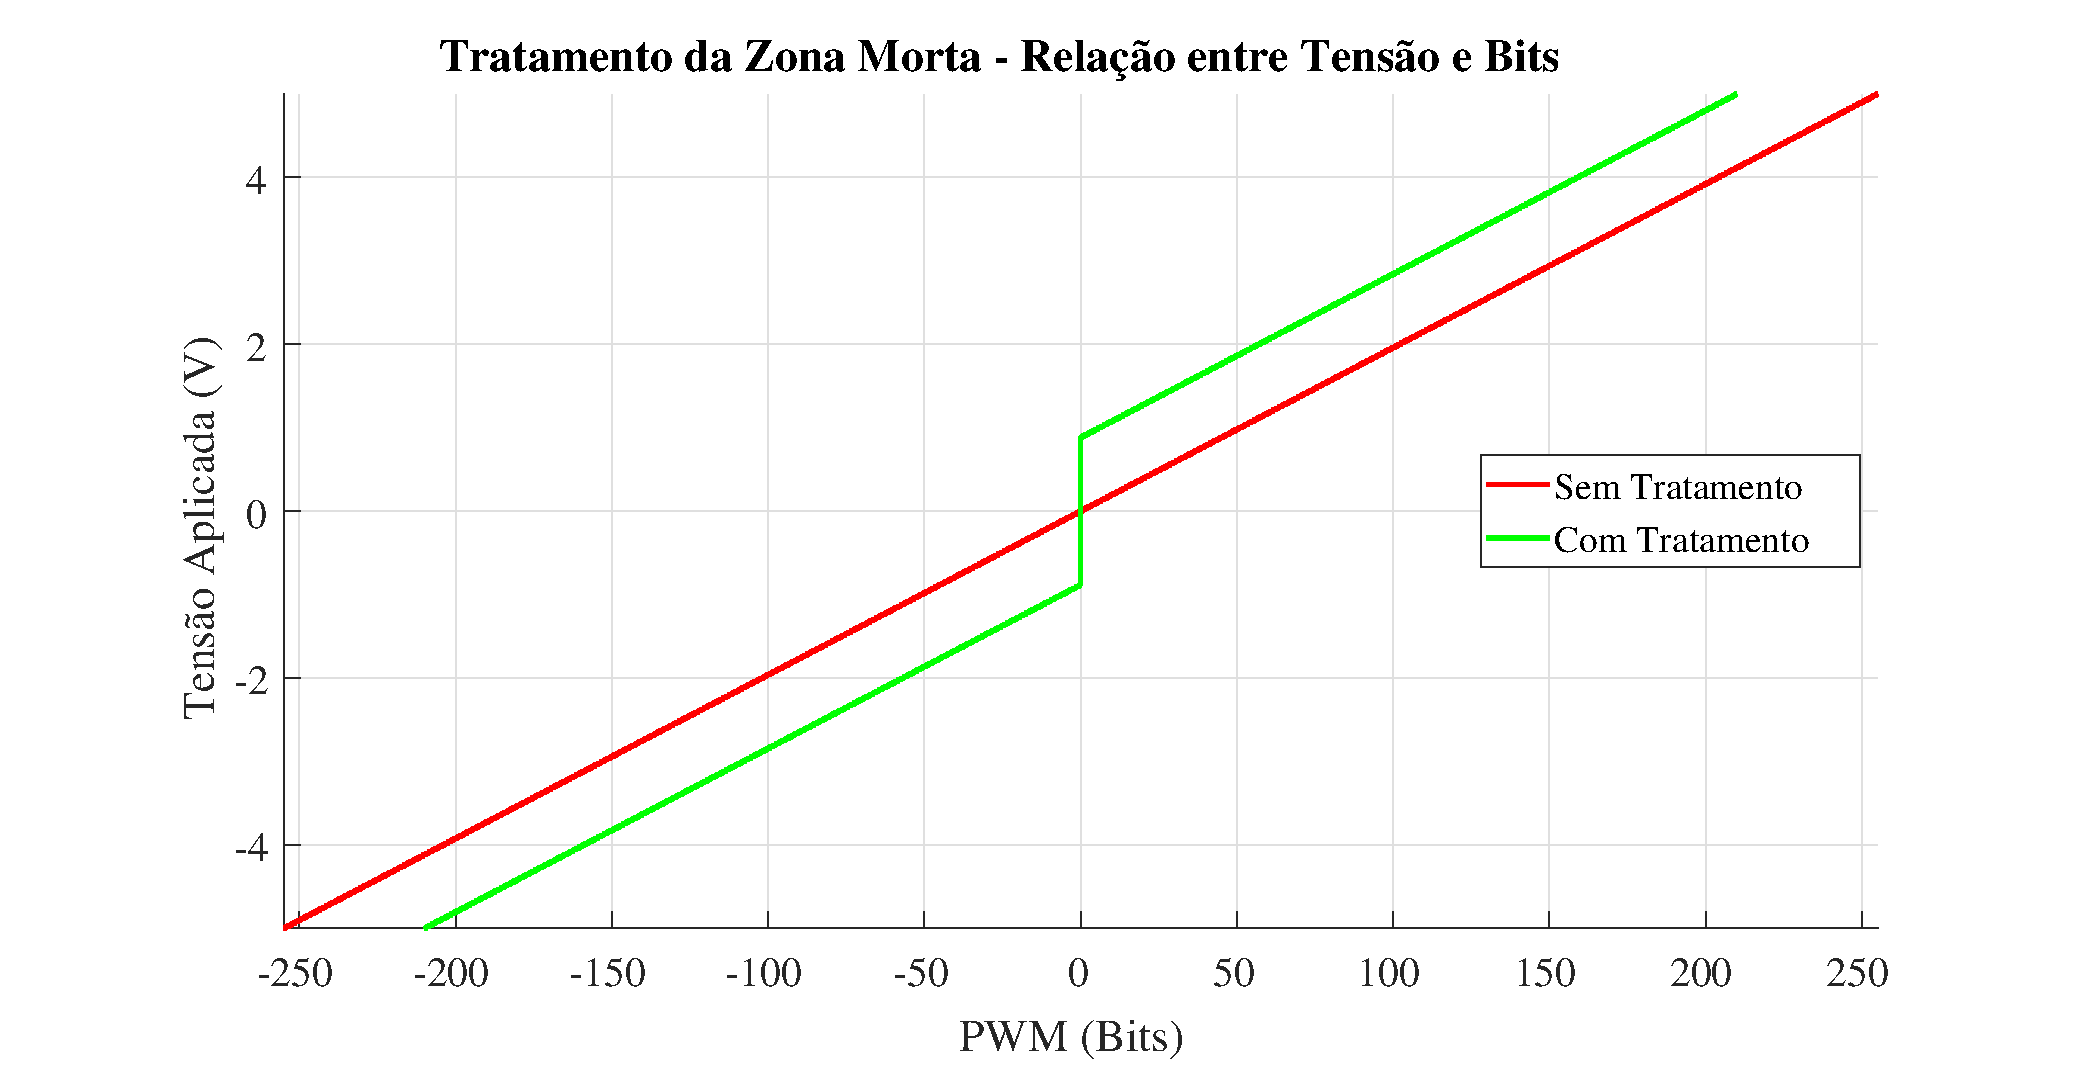
\includegraphics[width=\columnwidth]{imagens/zonamorta.eps}{
                    \small
                    \centering
                    \caption{Relação entre a tensão aplicada no atuador e bits de PWM, antes e depois do tratamento.}
                    \label{ZonaMorta}}
                \end{figure}
                
                Ficando assim a tabela de valores de entrada:
                
                \begin{table}[H]
                    \begin{tabular}{|
                        >{\columncolor[HTML]{C0C0C0}}l |c|c|c|}
                        \hline
                            \cellcolor[HTML]{C0C0C0}\textbf{Entrada} &
                            \cellcolor[HTML]{C0C0C0}\textbf{PWM (Bits)} &
                            \cellcolor[HTML]{C0C0C0}\textbf{\begin{tabular}[c]{@{}c@{}}Tensão (V)\end{tabular}} \\
                        \hline
                        \textbf{\begin{tabular}[c]{@{}l@{}}Mínimo \\(Real)      \end{tabular}} & -255 & -5      \\ \hline
                        \textbf{\begin{tabular}[c]{@{}l@{}}Máximo \\(Real)      \end{tabular}} &  255 &  5      \\ \hline
                        \textbf{\begin{tabular}[c]{@{}l@{}}Zona \\Morta         \end{tabular}} &  $\pm 45$ &  $\pm 1.078$  \\ \hline
                        \textbf{\begin{tabular}[c]{@{}l@{}}Mínimo \\(Tratado)   \end{tabular}} & -210 & -5      \\ \hline
                        \textbf{\begin{tabular}[c]{@{}l@{}}Máximo \\(Tratado)   \end{tabular}} &  210 &  5      \\ \hline
                        \textbf{\begin{tabular}[c]{@{}l@{}}Ponto de \\Operação  \end{tabular}} &    0 &  0      \\ \hline
                    \end{tabular}
                \end{table}
                
            \subsubsection{Faixa de valores de saída}
            
                O potenciômetro é acoplado diretamente ao eixo de saída da caixa de redução do motor. O sinal do potenciômetro vai para o DAC que o  converte para bits no intervalo de 0 a 1023. Abaixo a tabela de valores para a saída.
                
                \begin{table}[H]
                    \begin{tabular}{|
                        >{\columncolor[HTML]{C0C0C0}}l |c|c|c|}
                        \hline
                            \cellcolor[HTML]{C0C0C0}\textbf{Saída} &
                            \cellcolor[HTML]{C0C0C0}\textbf{DAC (Bits)} &
                            \cellcolor[HTML]{C0C0C0}\textbf{\begin{tabular}[c]{@{}c@{}}Angulo (\degree)\end{tabular}} \\
                        \hline
                        
                        \textbf{\begin{tabular}[c]{@{}l@{}}Mínimo               \end{tabular}} &    0 & -90     \\ \hline
                        \textbf{\begin{tabular}[c]{@{}l@{}}Máximo               \end{tabular}} & 1024 &  90     \\ \hline
                        \textbf{\begin{tabular}[c]{@{}l@{}}Ponto de \\Operação  \end{tabular}} &  512 &   0     \\ \hline
                    \end{tabular}
                \end{table}
                
                Via código é aplicado um \textit{offset} na leitura para deslocar o 0 bits para o 0\degree.

            \subsubsection{Identificação da Planta}
                
                Com o objetivo de identificar o modelo da planta aplicou-se o sinal \textit{Sweep Sine} na entrada do sistema e coletou a saída, como visto na Figura \ref{ident}. Utilizou-se o método de identificação do \textit{MatLab}, \textit{ident}, e obteve-se a seguinte função de transferência no domínio $s$:
                
                \begin{figure}[!htb] 
                \centering 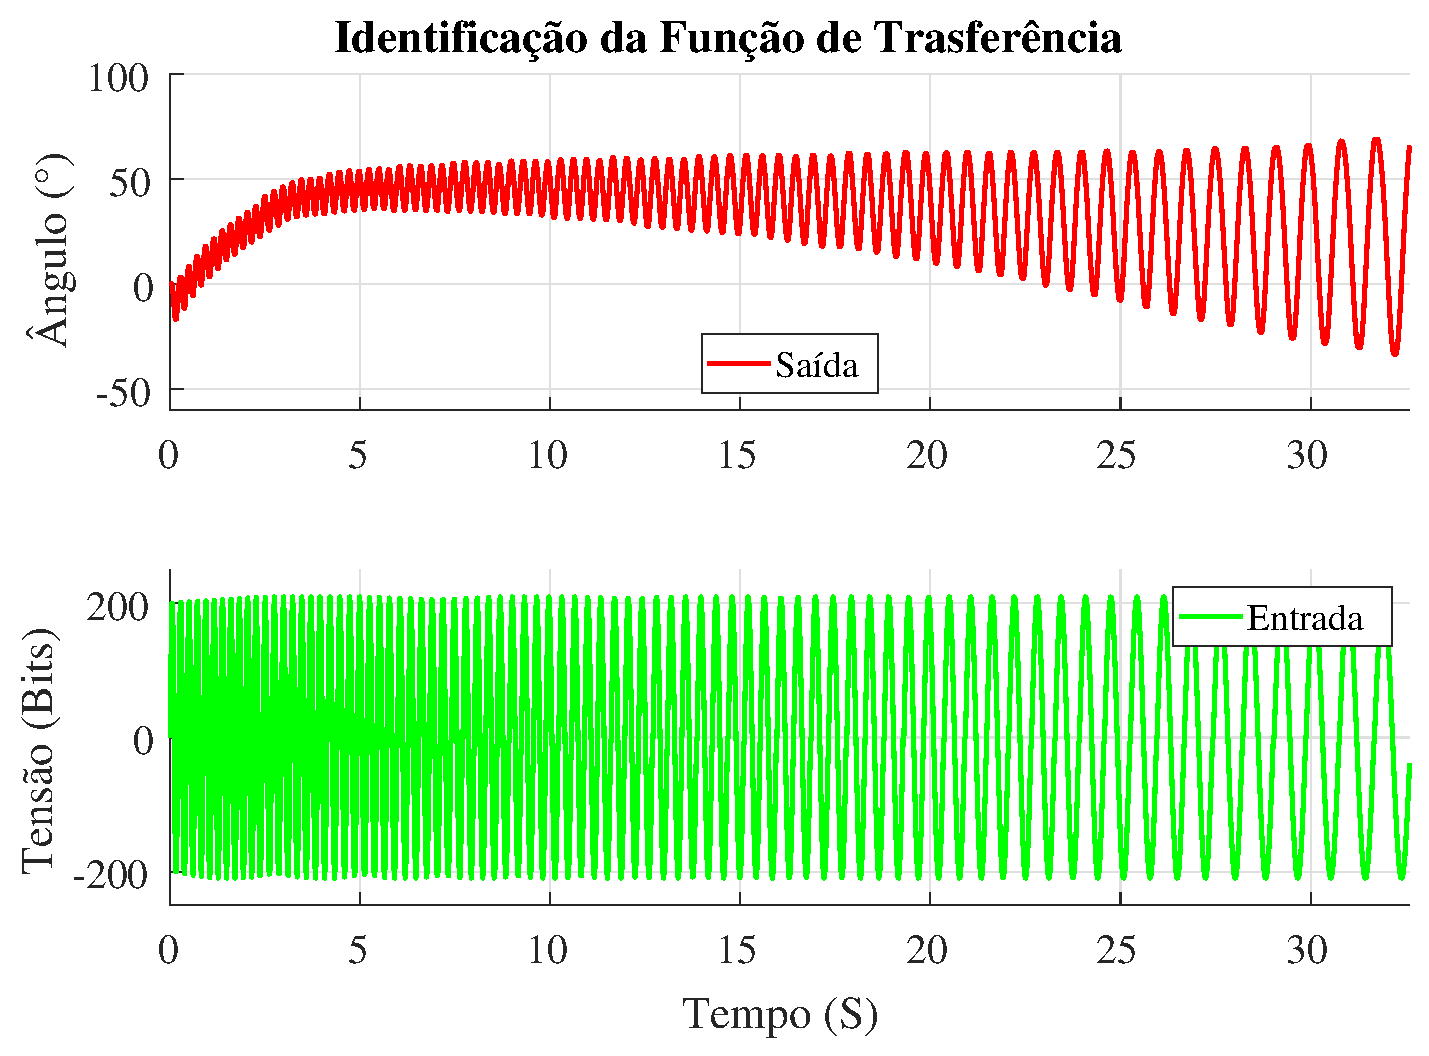
\includegraphics[width=\columnwidth]{imagens/ident.eps}{
                    \small
                    \centering
                    \caption{Identificação do Modelo da planta usando \textit{Sweep Sine}}
                    \label{ident}}
                \end{figure}
                
                \begin{equation}
                    G(s) = \frac{175}{s(s+17.5)}
                \end{equation}
                
                
                 
            \subsubsection{Validação do Modelo}
            
                A identificação do sistema contem erros induzidos durante o teste como não linearidades, arredondamentos, ruídos, pertubações externas, entre outros, portanto faz-se necessário validar a identificação. Para tal é preciso aplicar um sinal diferente do usado na identificação. 
                
                \begin{figure}[!htb] 
                \centering 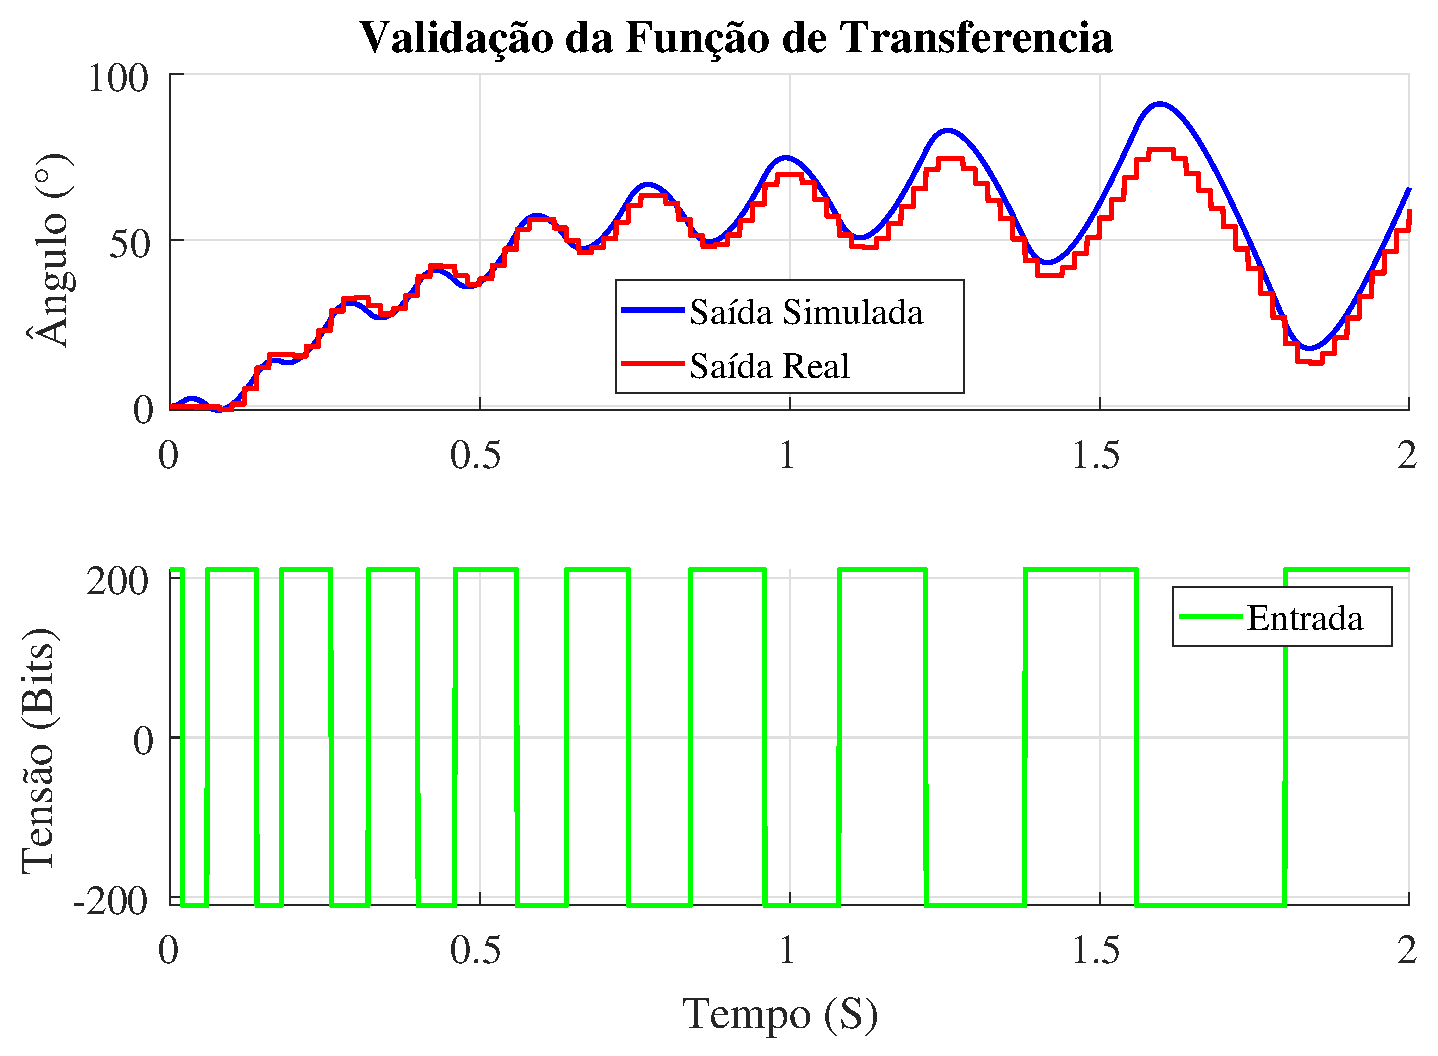
\includegraphics[width=\columnwidth]{imagens/valida.eps}{
                    \small
                    \centering
                    \caption{Relação entre a tensão aplicada no atuador e bits de PWM, antes e depois do tratamento.}
                    \label{ZonaMorta}}
                \end{figure}
                
    
            \subsubsection{Identificação da dinâmica de saturação}
                
                Como é necessário obter o menor tempo de acomodação dentro das possibilidades da planta, faz-se necessário identificar a dinâmica de saturação da planta a fim encontrar o limite de tempo de acomodação para uma determinada variação de interesse.
                
                O processo que demanda este sistema de controle varia em media $\pm35\degree$, então foi aplicado um pulso com uma duração que leva a aproximada $70\degree$. O resultado pode ser visto no gráfico abaixo.
                
                \begin{figure}[!htb] 
                \centering 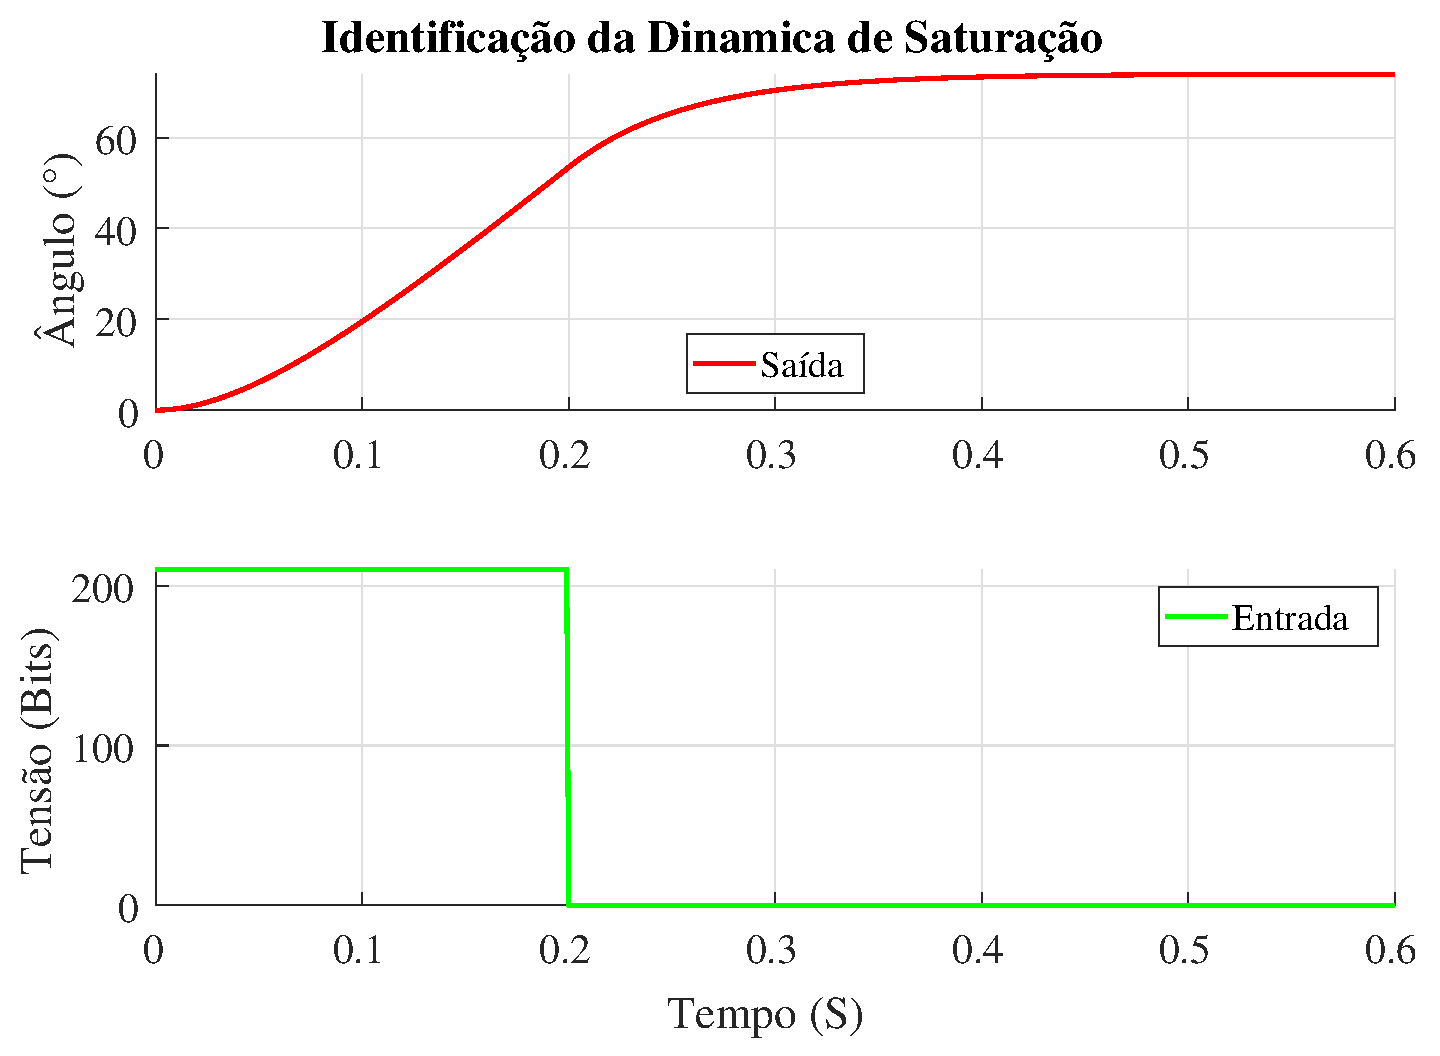
\includegraphics[width=\columnwidth]{imagens/sat.eps}{
                    \small
                    \centering
                    \caption{Saída da planta para uma entrada pulso com a amplitude de saturação.}
                    \label{ZonaMorta}}
                \end{figure}
                
                Pelo gráfico pode-se extrair o tempo de acomodação, que é aproximadamente $0,35s$.
                
        \subsection{Critérios de Desempenho Desejados}
            
            Para os projetos dos controladores especificou-se um tempo de acomodação de 0.4s, uma margem de 0.05s em relação ao tempo de acomodação com saturação, e \textit{overshoot} de no máximo $2\%$.
            
            Tais especificações geram polos desejados em:
            
            \begin{equation}
                s_{1,2} = -10 \pm 8.0306i
            \end{equation}
                
        \subsection{Plano Discreto}
            
            Com o tempo de acomodação especificada, escolheu-se a taxa de amostragem de $0.02s$ para discretizar o sistema. Discretizando o sistema com um ZOH, segurador de ordem zero, a função de transferência obtida:
                
            \begin{equation}
                G(z) = \frac{0.03125 z + 0.02781}{z^2 - 1.705 z + 0.7047}
            \end{equation}
            
            E obtendo o espaço de estados a partir de G(s) e depois discretizando-os, obteve-se as seguintes matrizes:

            \begin{equation}
                A =
                \begin{bmatrix} 0.704294786861096 & 0
                            \\  0.016870530849940 & 0.002856672307105
                \end{bmatrix}
            \end{equation}
            
            \begin{equation}
                B = 
                \begin{bmatrix} 0.269928493599033
                            \\  0.002856672307105
                \end{bmatrix}
            \end{equation}
            
            \begin{equation}
                C = \begin{bmatrix} 0 & 9.163685739927198
                \end{bmatrix}
            \end{equation}
            
            \begin{equation}
                D = 0
            \end{equation}
                
            Discretizou-se os polos desejados e obteve-se:
            
            \begin{equation}
                z_{1,2} = 0.8082 \pm 0.1309i
            \end{equation}
            
            A Figura \ref{LGR} apresenta o Lugar Geométrico das Raízes com o posicionamento do polo desejado, marcado em vermelho.
            
            \begin{figure}[!htb] 
                \centering 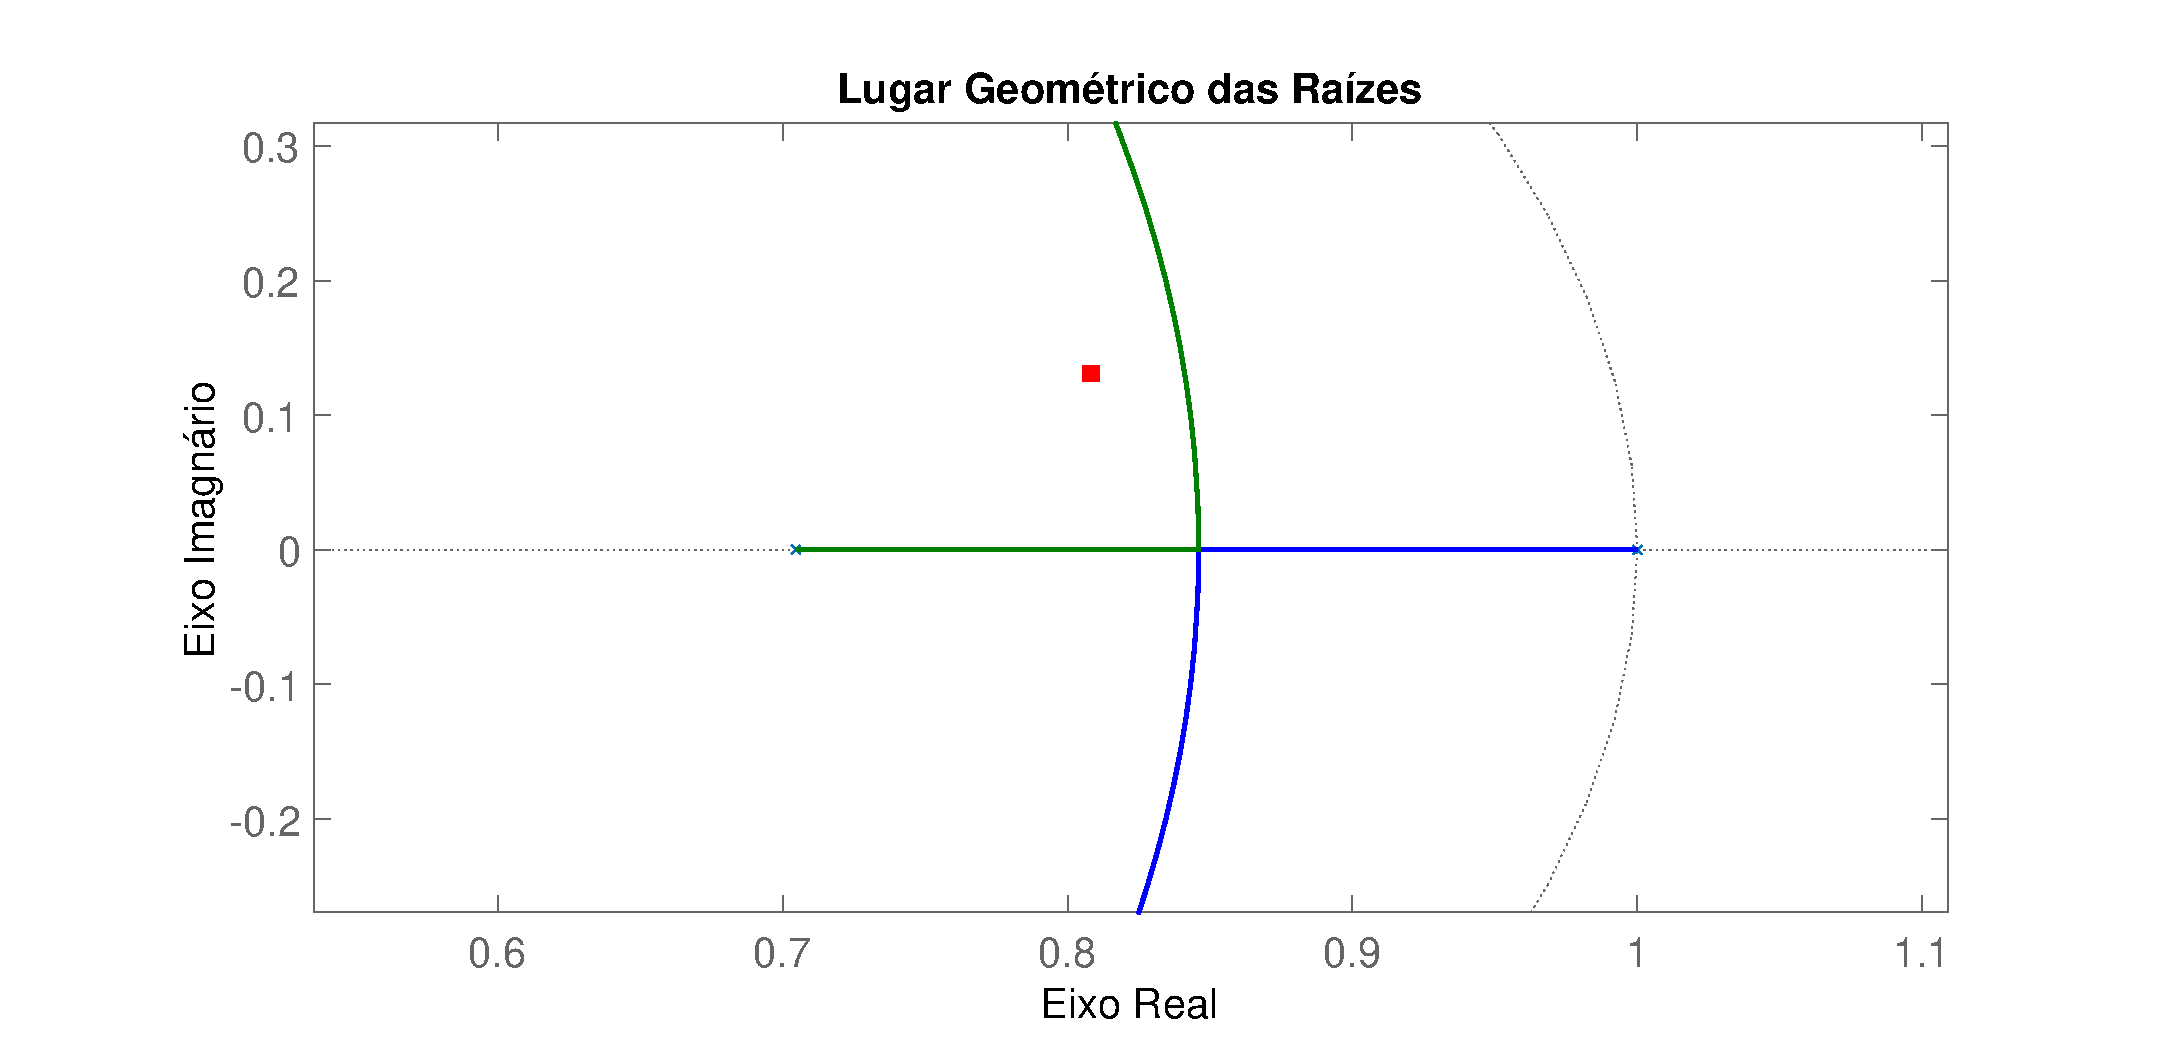
\includegraphics[width=\columnwidth]{imagens/lgr.eps}{
                    \small
                    \centering
                    \caption{Lugar Geométrico das Raízes com o polo desejado, em vermelho.}
                \label{LGR}}
            \end{figure}
        
        \subsection{Projeto de um controlador PID pelo método Lugar das Raízes}
        
            Como o Lugar Geométrico das Raízes não passa pelas especificações desejadas, projetou-se um controlador PID utilizando o método do Lugar Geométrico das Raízes. Pode ser observado o Lugar Geométrico das Raízes do modelo com PID projetado na Figura \ref{LGRPID}.
            
            \begin{equation}
                C(z)=\frac{2.092z^2-3.114z+1.024}{z^2-z}
            \end{equation}
            
            Encontrou-se os valores para os ganhos do PID de:
            
            \begin{equation}
                K_P=1.06517
            \end{equation}
            
            \begin{equation}
                K_D=1.0246
            \end{equation}
            
            \begin{equation}
                K_I=0.0011
            \end{equation}
            
            \begin{figure}[!htb] 
                \centering 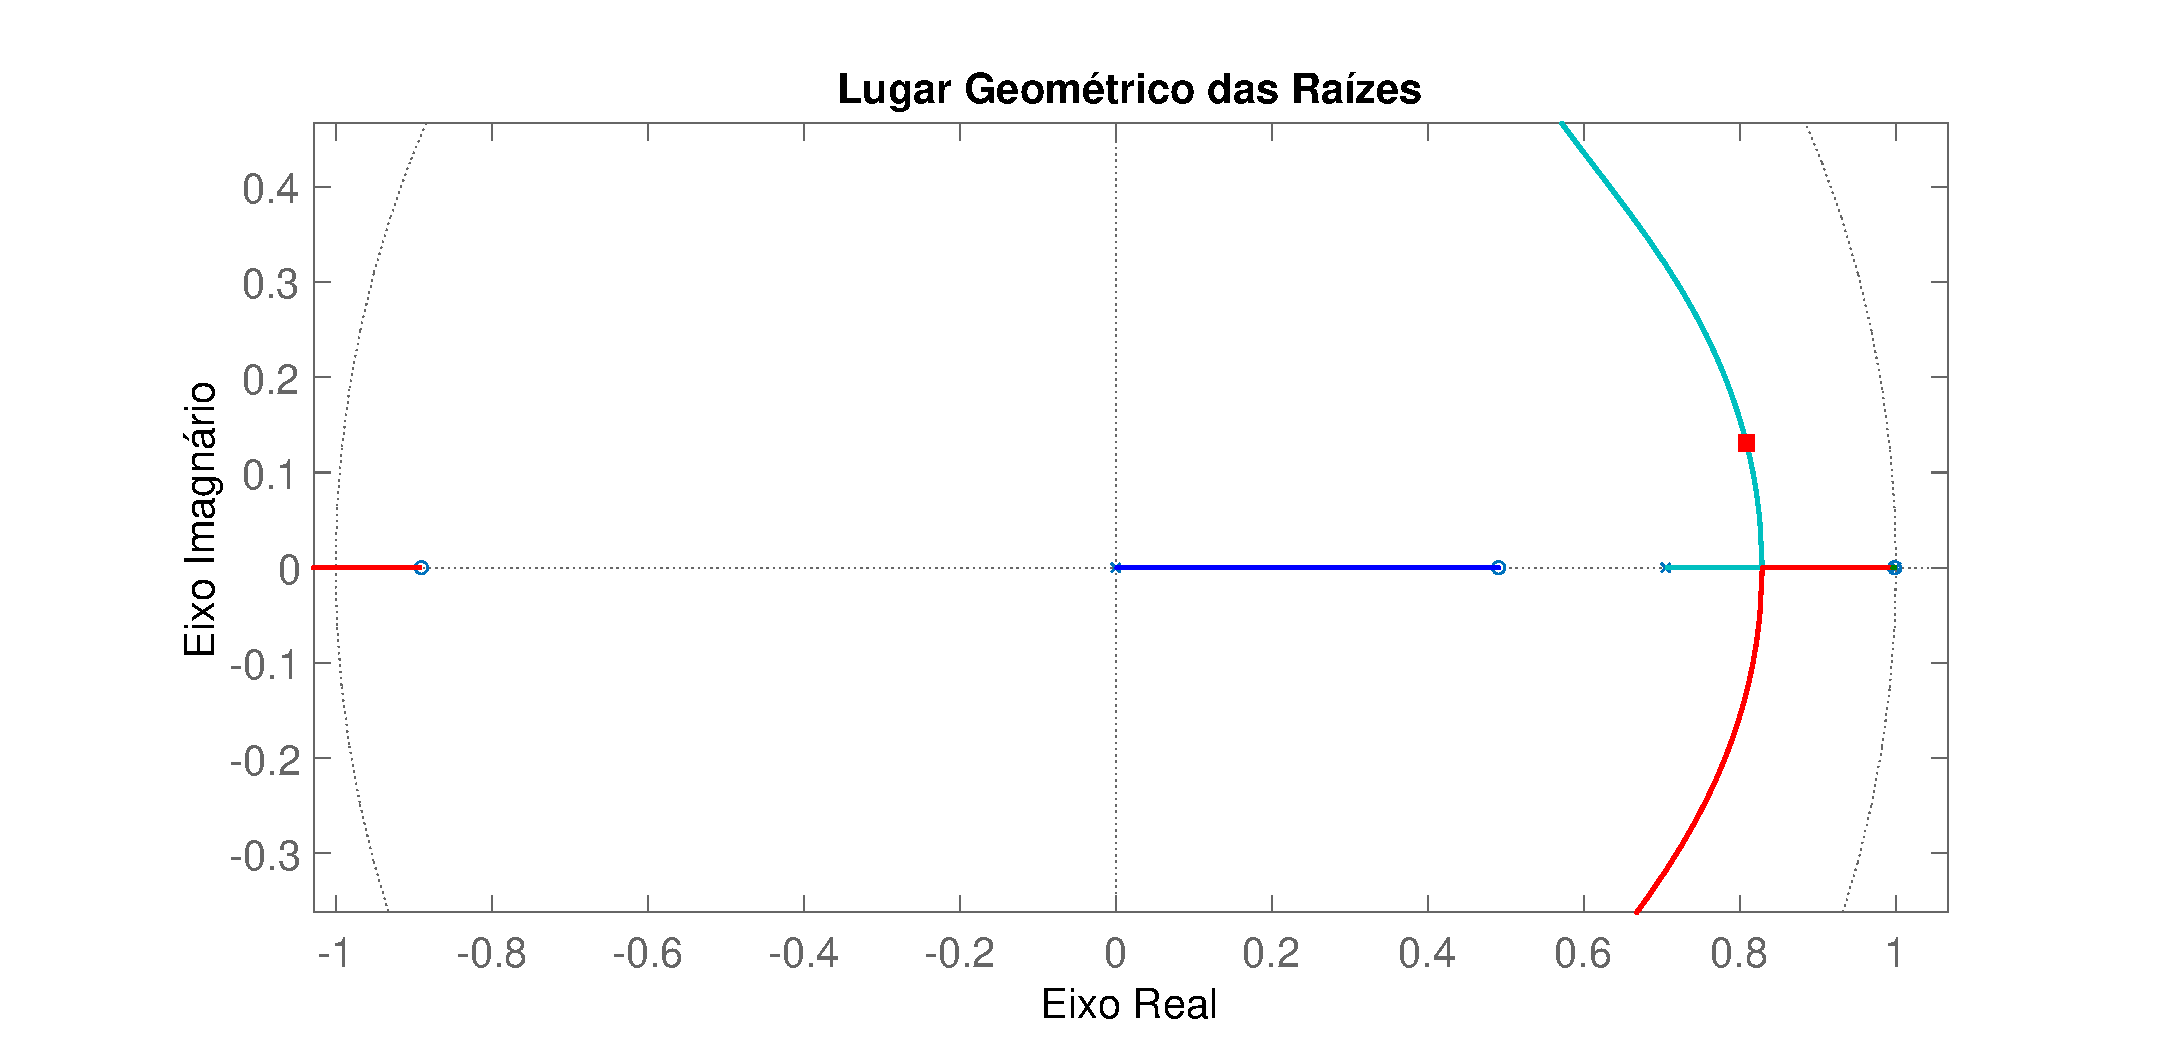
\includegraphics[width=\columnwidth]{imagens/lgrPID.eps}{
                    \small
                    \centering
                    \caption{Lugar Geométrico das Raízes do modelo com PID, polo desejado em vermelho.}
                    \label{LGRPID}}    
            \end{figure}
            
        \subsection{Projeto de um controlador e observador por Realimentação de Estados pelo método da Alocação de Polos}
        
            Para projetar o controlador por REE, projetou-se um controlador, com integrador, e um estimador de estados.
                
            Para o projeto, especificou-se os polos desejados, tanto do controlador - de acordo com a dinâmica desejada - quanto para o observador - sendo 10x mais rápidos que os do controlador.
            
            Para o controlador com a adição do efeito integral, necessitou-se adaptar as equações \ref{ackermann_controla} e \ref{controlabilidade} e acrescentar um outro polo, 10x mais rápido que a dinâmica desejada no contínuo.
            
            Com as adaptações, as equações podem ser escritas como:
            
            \begin{equation}
                \begin{bmatrix}K & -K_a\end{bmatrix}= \begin{bmatrix}
                    0 & 0 & 1
                \end{bmatrix}
                \textbf{C}^{-1}\Delta_d(A_a)
                \label{aumentada}
           \end{equation}
           
           \begin{equation}
               \textbf{C}= \begin{bmatrix}
                    B_a & A_aB_a & A_a^2B_a
               \end{bmatrix}
           \end{equation}
           
           sendo
           
           \begin{equation}
               A_a=
                    \begin{bmatrix} A & 0
                                \\  -CA & 1
                    \end{bmatrix}
           \end{equation}
           
           \begin{equation}
               B_a=
                    \begin{bmatrix} B & -CB
                    \end{bmatrix}
           \end{equation}
           
           Para o observador utilizou-se:
           
           \begin{equation}
                L=\Delta_d(A)\textbf{O}^{-1}
                \begin{bmatrix}
                    0\\ 
                    1
                \end{bmatrix}
                \label{observador}
            \end{equation}
            
            Onde
            
            \begin{equation}
                \textbf{O}=\begin{bmatrix}
                C\\
                CA\\
                \end{bmatrix}
            \end{equation}
            
            Utilizando a equação \ref{aumentada} e \ref{observador} encontrou-se os valores de ganhos:
           
           \begin{equation}
               K=\begin{bmatrix}2.741950191395121 & 65.124363946536870\end{bmatrix}
           \end{equation}
           
           \begin{equation}
               K_a=0.913877825841094
           \end{equation}
           
           \begin{equation}
               L=\begin{bmatrix}0.610653949032228\\
               0.097788322092752\end{bmatrix}
           \end{equation}
           
            
            
            
        
    
    \section{Resultados e Discussões}
    
        \subsection{Sistema de malha fechada com controlador PID}
        
        
            As figuras \ref{PID_n_sat} e \ref{PID_sat} representam os sinais de saída e controle com o sinal de controle não saturado e saturado, respectivamente, da planta e simulação com um controlador PID.
        
            \begin{figure}[!htb] 
                \centering
                    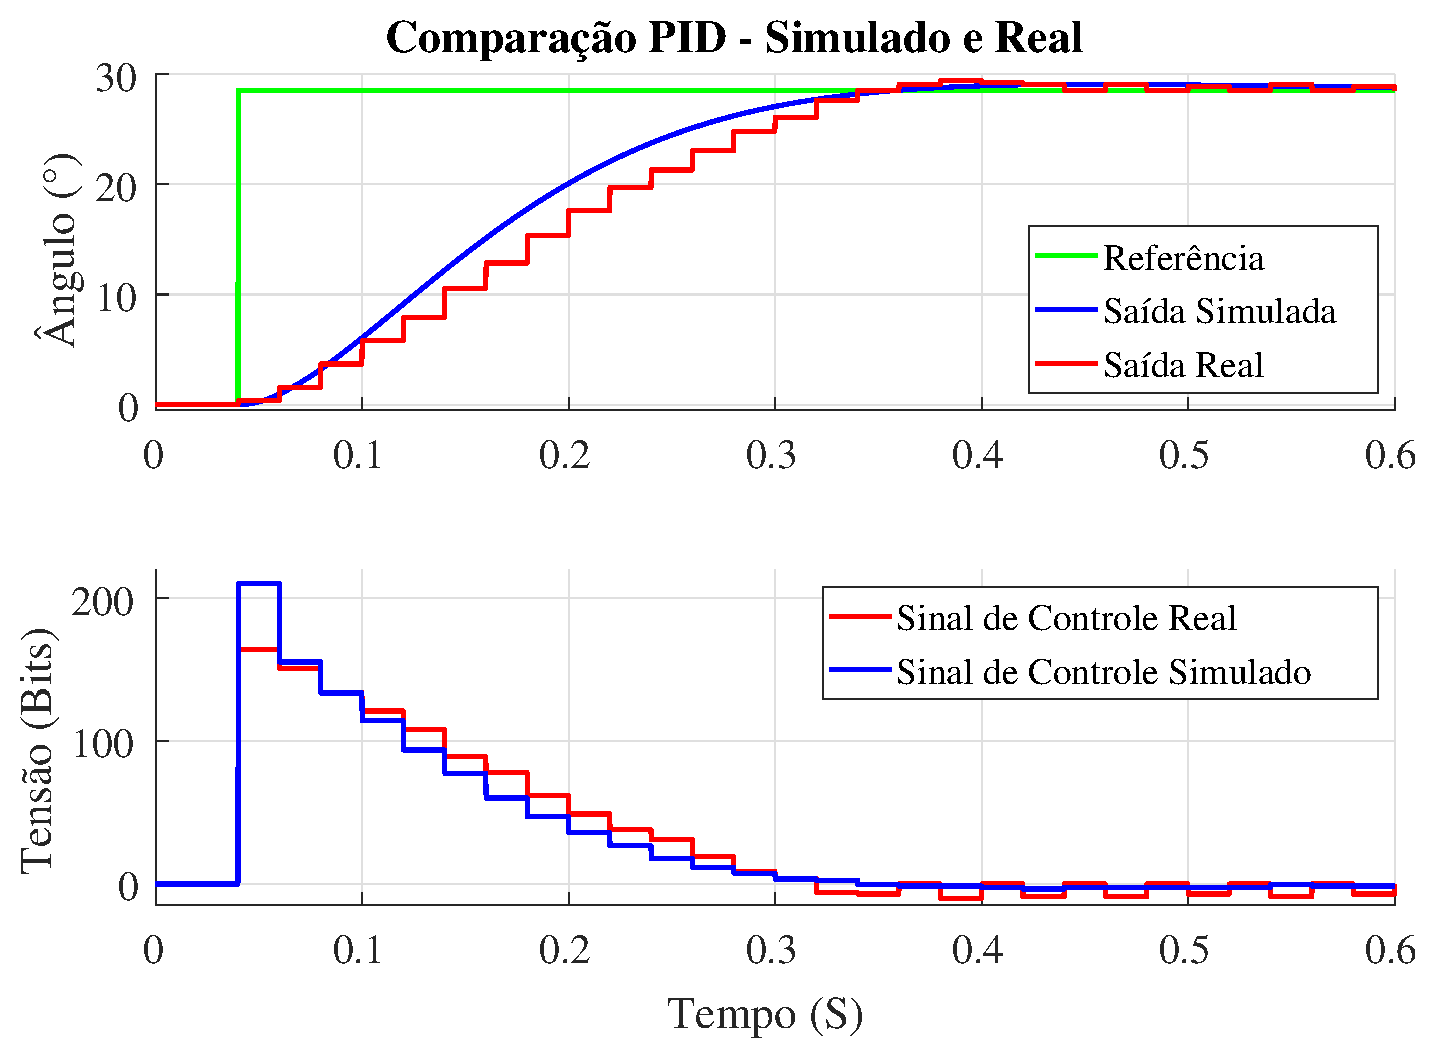
\includegraphics[width=\columnwidth]{imagens/malhafechada/SimuRealPIDnSat.eps}{
                    \small
                    \centering
                    \caption{Resposta e Sinal de Controle com Controlador PID}
                    \label{PID_n_sat}}
            \end{figure}
        
            \begin{figure}[!htb] 
                \centering
                     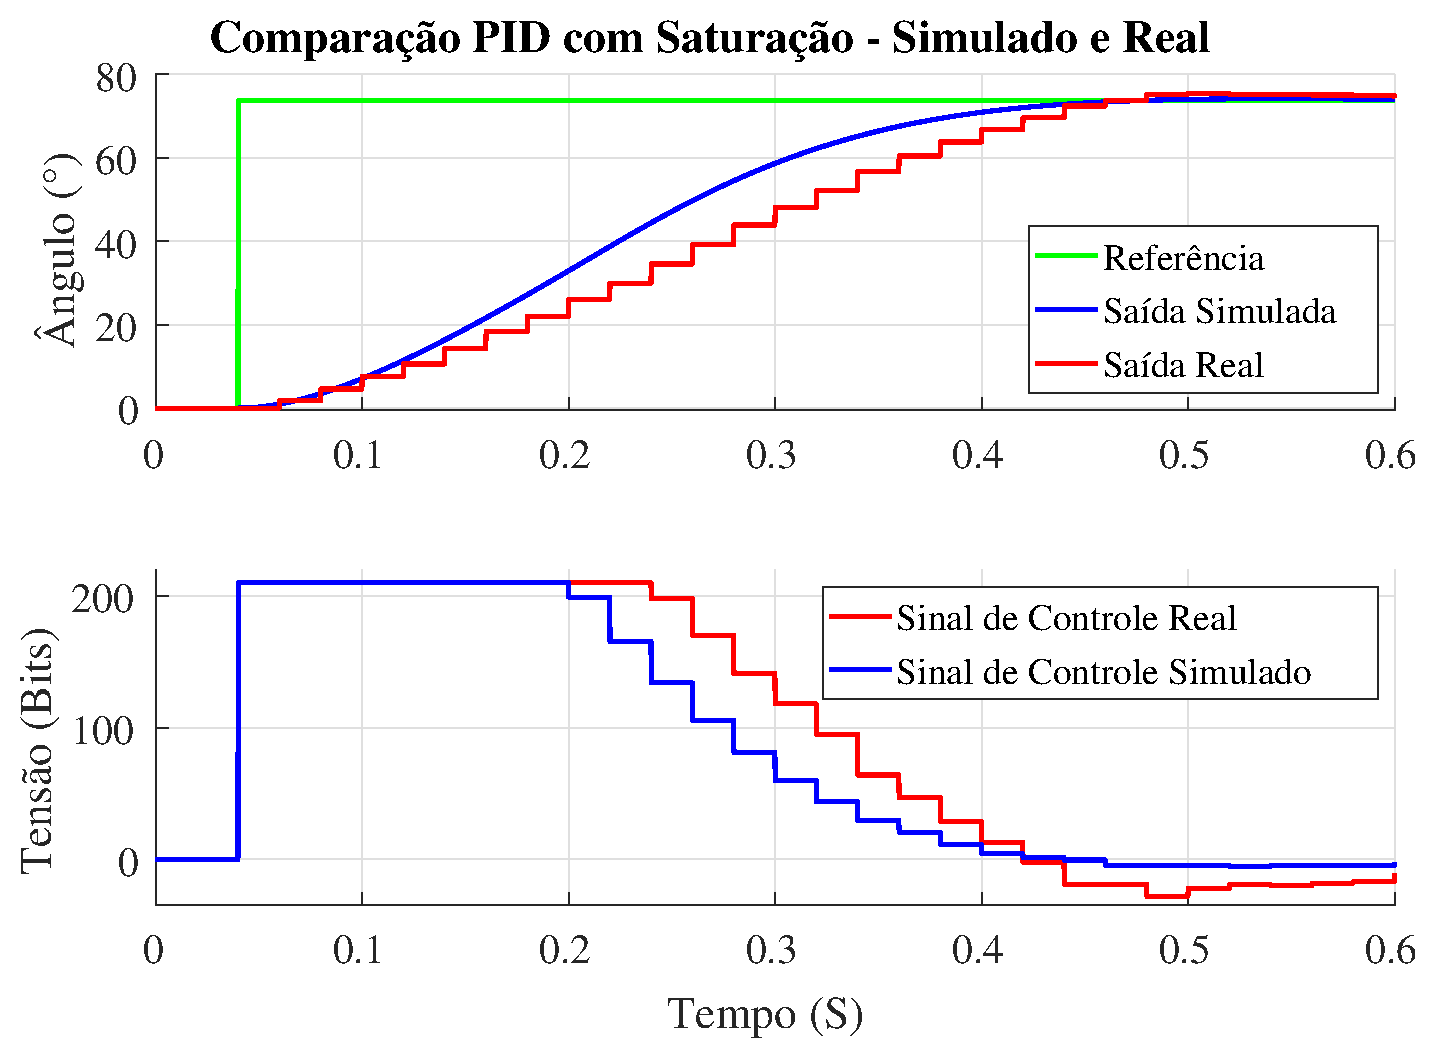
\includegraphics[width=\columnwidth]{imagens/malhafechada/SimuRealPIDsat.eps}{
                    \small
                    \centering
                    \caption{Resposta e Sinal de Controle com Controlador PID - Saturado}
                    \label{PID_sat}}
            \end{figure}
        
        
        
        \subsection{Sistema de malha fechada com controlador REE.}
        
        
        
            As figuras \ref{SS_n_sat} e \ref{SS_sat} representam os sinais de saída e controle não saturado e saturado do sistema, respectivamente, da planta e simulação com REE.
        
            \begin{figure}[!htb] 
                \centering
                    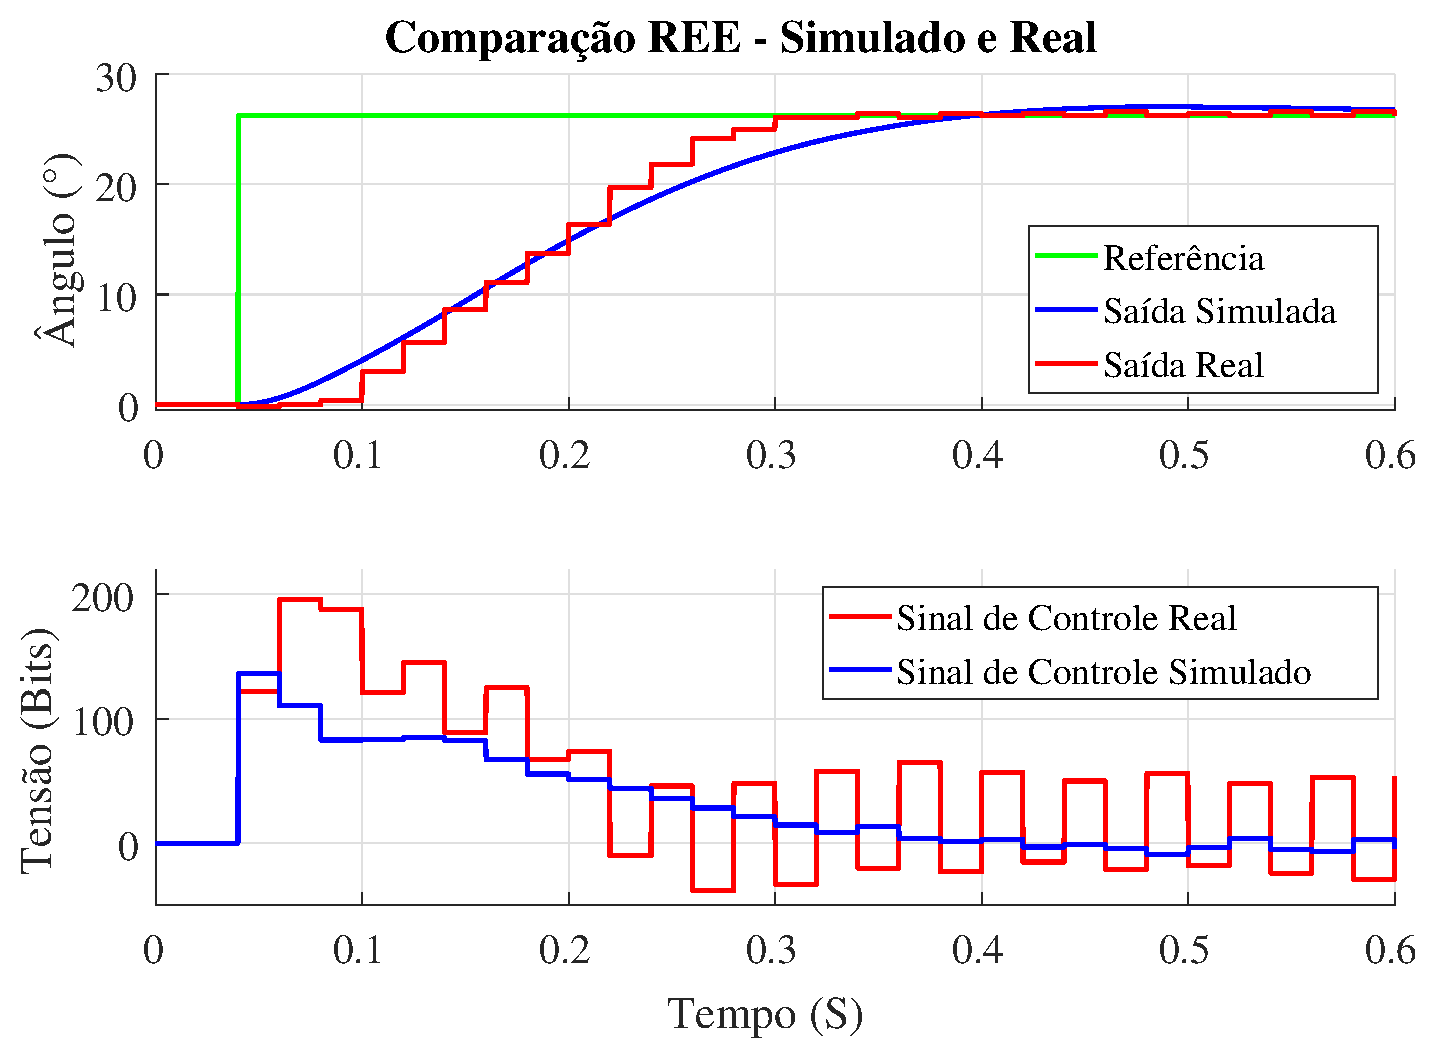
\includegraphics[width=\columnwidth]{imagens/malhafechada/SimuRealSSnSat.eps}{
                    \small
                    \centering
                    \caption{Resposta e Sinal de Controle com REE.}
                    \label{SS_n_sat}}
            \end{figure}
            
            \begin{figure}[!htb] 
                \centering
                    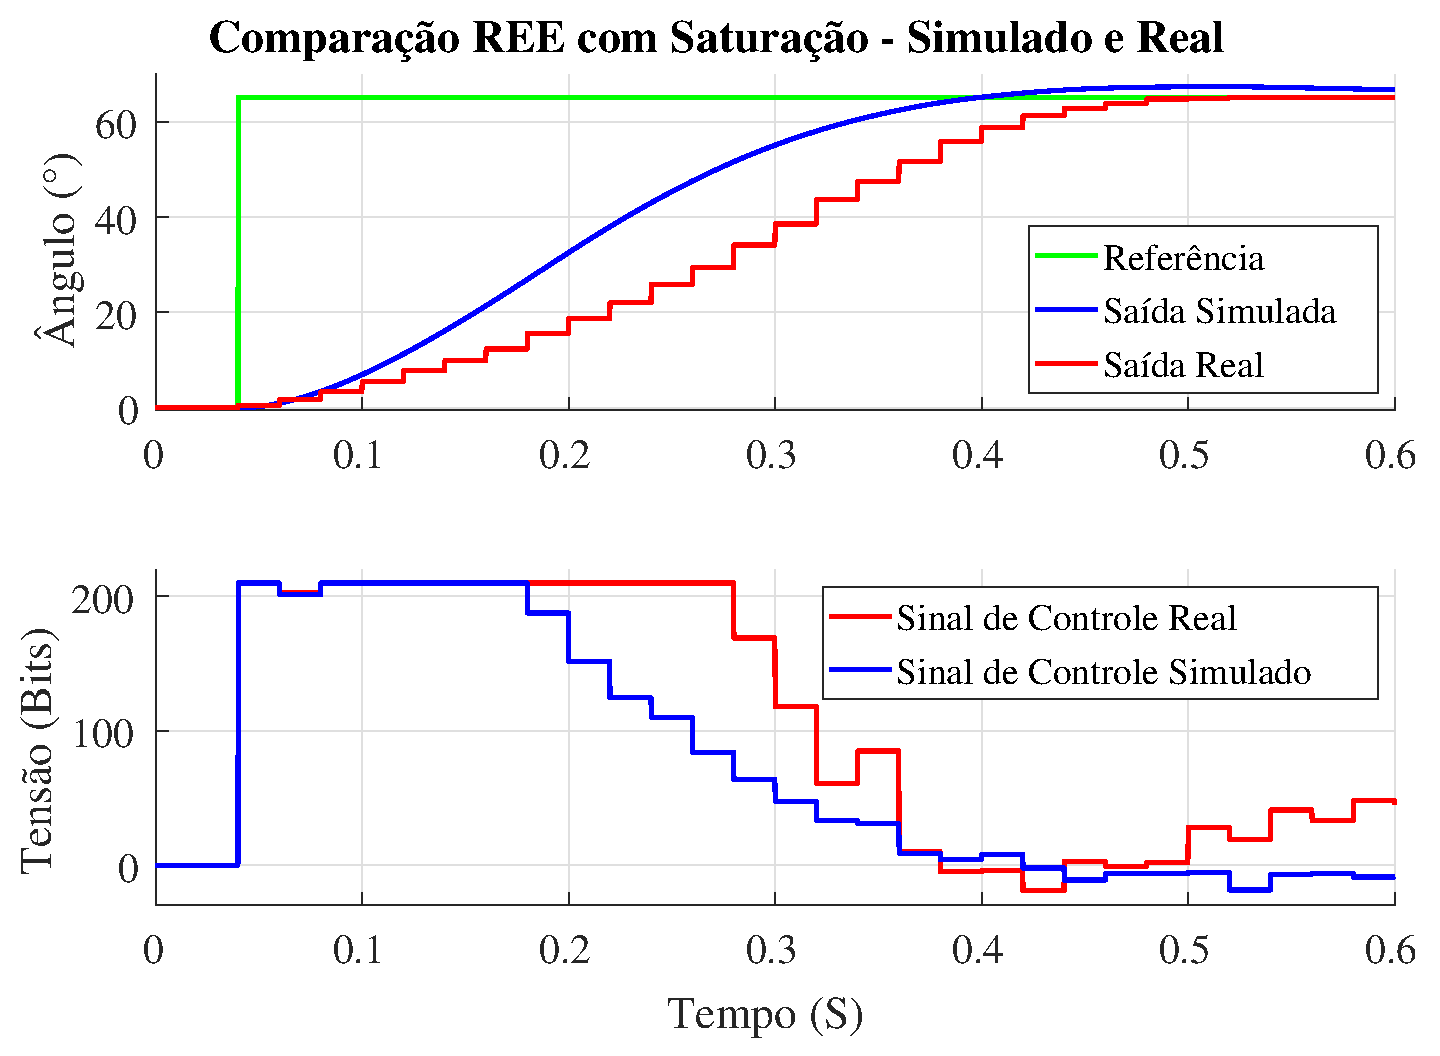
\includegraphics[width=\columnwidth]{imagens/malhafechada/SimuRealSSsat.eps}{
                    \small
                    \centering
                    \caption{Resposta e Sinal de Controle com REE - Saturado}
                    \label{SS_sat}}
            \end{figure}
        
        \subsection{Discussões}
            As respostas de ambos os controladores sem apresentar saturação apresentam uma dinâmica similar com a simulação. Além disso, a resposta da planta com o controlador REE apresentou uma resposta mais rápida que o controlador PID. Entretanto, quando simulada com a saturação prevista, a planta apresentou um tempo de acomodação um pouco maior que o da simulação.
        
        
    \section{Considerações Finais e Propostas Futuras}
    
        Futuramente quando ser realizado o controle de inclinação da planta sera feito os testes para ver se os critérios de desempenho estão satisfatórios para o mesmo. Caso não for, será necessário realizar a troca de alguns componentes, como a caixa de redução com menos folgas.
        
    \nocite{*}
    \bibliography{referencias.bib}
    
    
\end{document}